\section*{Reactor design}
Transitioning from batch to continuous process requires a complete redesign of the reactors that are commonly used in the industry today. Nitroma developed a novel approach of using a Heat Exchanger Reactor (HEX Reactor) for the nitration of toluene. The reactor handles 816 tonnes of ONT and 841 tonnes of PNT throughput per annum. 

%kinetics and general overview [zong]
The kinetics of the zeolite-catalysed nitration reaction was determined using literature data and the Arrhenius equation. Instead of assuming the same rate equation for all 3 nitrotoluene
- SiC immobilise
%modelling approach [andreas]
The model was implemented and optimised on COMSOL 5.6. 
-steps taken to model ( Brinkman) 

%optimisation [zong]
To ensure the reactor operates in optimal conditions, the following parameters were optimised: Concentric inner cooling pipe diameter and flowrate, direction of cooling water flow, \ch{HNO3} : Toluene inlet ratio and the total number of reaction tubes.



A further sensitivity analysis was performed on the cooling water inlet temperature since the temperature inside the reactor needs to be well-controlled at all times. Cooling water temperature was simulated to vary by \mypm $\Delta$ 5 K and the total length of reactor required to achieve 98\% conversion while keeping temperature below the safe limit of 363K was investigated. The cooling water is not expected to fluctuate to this degree since it is reused and mixed together from multiple cooling water streams in the plant, but taking a conservative approach increases the overall safety of Nitroma's plant in the worst case scenario. The optimal length was determined to be 4.2m. 


%mech design [loon]
\begin{figure}[h]
    \centering
    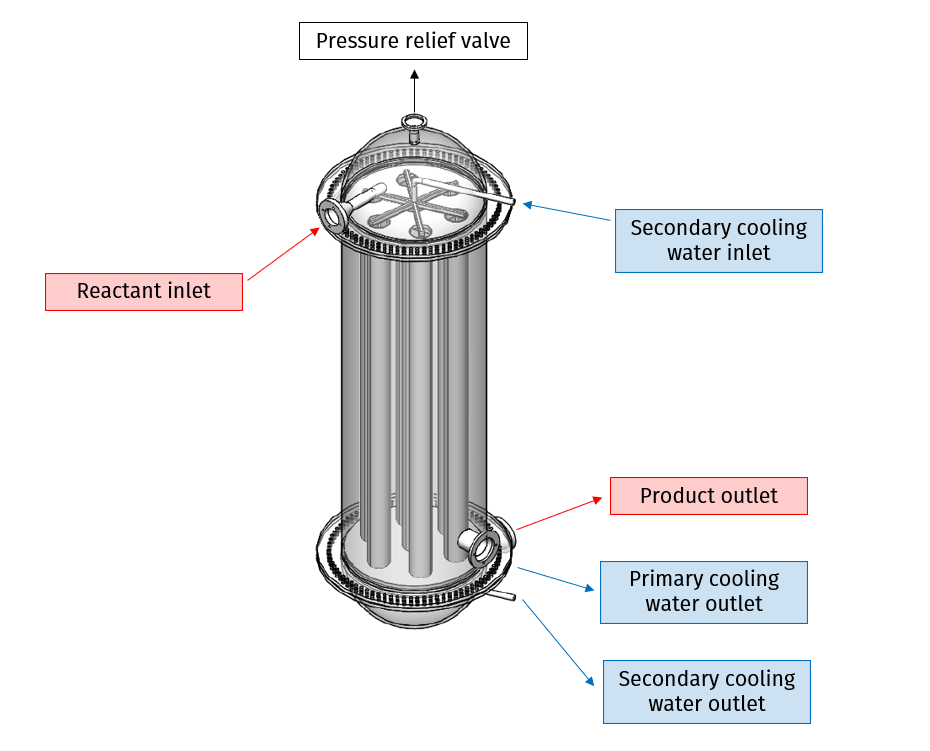
\includegraphics[width=0.7\linewidth]{chapters/0-executive-summary/figures/FYD executive sum.PNG}
    \caption{Mechanical design of nitration reactor}
    \label{fig:executivesummaryreactor}
\end{figure}